
\chapter{Bitcoin Point of Sale Terminals: Evaluation and Deployment}

%==================== Introduction ======================

\section{Introductory Remarks}

In previous chapter we evaluated all the existing Bitcoin wallet clients for the user. In this chapter we survey and evaluate the existing Bitcoin payments for a business to accept Bitcoin and use SCRAM~\cite{REScenario}  requirement engineering method to develop the most suitable Point of Sale (PoS) for a small business based on our evaluation framework. We would use PoS for point of sale terminal through out this chapter. Even though we borrowed some concepts used in the previous chapter, we introduce new concepts and build a new framework to evaluate Bitcoin point of sales.

One aspect of Bitcoin is that there is no specific entity backing up the currency, whoever that is using Bitcoin gives value to it. As a Bitcoin enthusiast one of the goals is to have more places to accept Bitcoin, however this has been an issue for the business owners to implement a simple, yet fully functional PoS to be able to accept Bitcoin as a method of payment.
This chapter discusses the approach we use to evaluate existing Bitcoin point of sales, our proposed approach, and the implementation of Aunja PoS in a Cafe in Montreal\footnote{ Cafe Aunja \url{http://aunja.com}}.

In order to do so, we started by eliciting the requirements of a payment system for a small business, and then researched the available options to see if they meet our requirements. Then, we put together a framework to compare these PoS with different criteria in security, privacy, usability and deployability categories. In the end, we implemented Aunja PoS for this small business that could be used in any other similar businesses as the payment method to accept Bitcoin.

%==================== Requirement ======================
\section {Requirments Engineering}
Requirement engineering is the process of defining, documenting and maintaining requirements and is a subfield of software and system engineering. The term was first used in 1979 ~\cite{alford1979software} and then became a general term with the publication of an IEEE Computer Society tutorial ~\cite{dorfman1990system}.
Requirements Engineering is the first phase in waterfall software development process ~\cite{rocye1970managing}. Depending on the type of the system being developed, the methods differ.

Probably the best way to analyze the requirements of a small business is to model real world descriptions and stories in scenarios. Scenarios are examples of real world experiences that we could use to model what is needed in the system. That is why scenario-based requirements engineering method named SCRAM was chosen.

\subsection{SCRAM}
We used SCRAM (Scenario-based Requirements Analysis Method) as our framework to gather the requirements of this system.
SCRAM defines four phases of requirement engineering and has been shown to be a great requirement engineering framework.


\begin{figure}[htb!p]
\centering
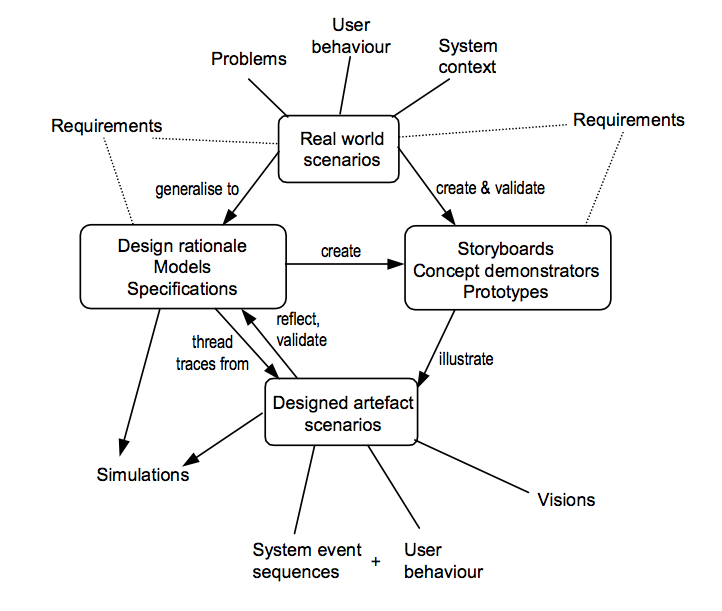
\includegraphics[width=\linewidth]{fig/REscenario.png}
  \caption{Role of scenarios and their relationship to requirements specifications and prototypes ~\cite{REScenario}}
\label{fig:REscenario}
\end{figure}


This method consists of four phases:
\begin{itemize}

\item \textbf{Initial requirements capture and domain familiarisation: } This is done by interviewing and fact-finding methods to have a full understanding of how the business works.

\item \textbf{Storyboarding and design visioning: } This is done by making storyboards and walkthroughs to show to the business and get feedback on feasibility.

\item \textbf{Requirement exploration: } This uses the early prototypes  and designs to get critiques from the business and validate the requirements.

\item \textbf{Prototyping and requirement validation: } This is done by developing fully functional prototypes and continues refining the requirements until the product is acceptable by the business.

\end{itemize}

%-------------------------- Initial requirements capture and domain familiarisation. --------------------------
\textit{Phase 1: Initial requirements capture and domain familiarisation.} We asked the cafe owner, two employees and two customers for a scenario involving Bitcoin payment in the cafe to create the common "normal use case". The differences between the scenarios were insignificant thus the exceptions to this normal use case are not valid. One exception was power failure, and because even the current accepted payment methods such as Visa would fail, it was not considered as a valid scenario, that being said, there are methods to mitigate this that will be discussed later in the thesis such as browser-based PoS.


As the cafe already have other payment systems in place, there is no need to go through the cafe's business plan or any other specification to check for conflicts. The only change is to implement another payment system at cashier's desk (see figure \ref{fig:phase1}).
However, there are requirements in the PoS system that need to be met, such as realtime Bitcoin to fiat money exchange and obvious alert of successful or failed payments.

\begin{figure}[htb!p]
\centering
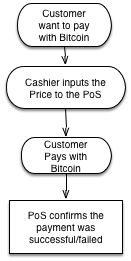
\includegraphics[scale=0.7]{fig/RE_Scenario_Phase1.png}
  \caption{Phase 1 - Normal Use Case}
\label{fig:phase1}
\end{figure}

%-------------------------- Storyboarding and design visioning --------------------------

\textit{Phase 2: Storyboarding and design visioning.}
Based on the information gathered from Phase 1 and further analysis, such as user survey on the design, storyboard was developed, see figure \ref{fig:storyboard}.% More technical requirements will be explained later ~/ref{section}.

%FIXME: wrapfigure package ! size
\begin{figure}[htb!p]
\centering
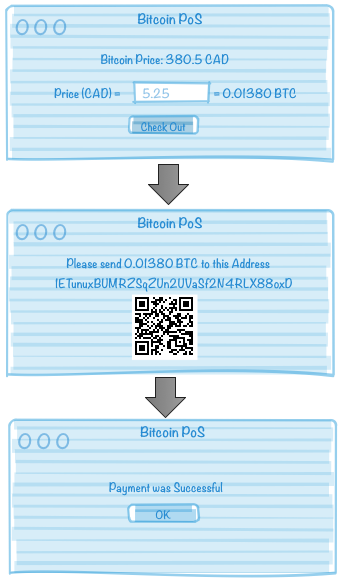
\includegraphics[scale=0.5]{fig/RE_Scenario_Interface.png}
  \caption{Storyboard - User Interface first sketch}
\label{fig:storyboard}
\end{figure}


%-------------------------- Requirements exploration. --------------------------
\textit{Phase 3: Requirements exploration.}
We developed a proof of concept\footnote{concept demonstrator~\cite{REScenario}} , capable of doing a simple Bitcoin payment. The Bitcoin exchange rate and the amount of transactions were hard coded and the transaction would be executed manually. We asked the employees to run a mock purchase with the demonstrator to see how they would interact with the system and received feedback. As Bitcoin concepts might be ambiguous for the new user, there should not be any interactions with Bitcoin concepts and terminology. After the transaction was done, the owner pointed that there is the need for a central logging system that could be checked from time to time for the daily transactions.\\


%-------------------------- Prototyping and requirements validation. --------------------------
\textit{Phase 4: Prototyping and requirements validation.}
We used the feedback gathered from phase 3 to make the first prototype. The prototype retrieved the Bitcoin exchange rate in realtime and the employee only had to input the dollar amount in the PoS. This made it possible to keep the Bitcoin terminology out of the scope of the training for the employees. However on the first prototype, to show the successful payments, the system was showing the transaction on a Blockchain explorer\footnote{\url{http://blockchain.info}}, using web-based APIs. This was not clear for a novice user on what the state of the system is. On the second round of prototyping, we designed an interface to show that the transaction has been broadcasted to the Bitcoin network and would use that knowledge to inform the employee of the state of the payment.\\

\section{Decision Framework}
We propose a framework specialized for Bitcoin point of sale systems to score the system with a set of requirements based on usability, deployability, privacy and security. These are not a final set of requirements for a general purpose system, however in the case of Bitcoin payments for a small business these will suffice. It worths mentioning that these requirements are a subset of Systems and Software Quality Requirements known as ISO/IEC 25010:2011 ~\cite{iso25010}. \\

We start by using our scenario based requirement engineering approach and adding the required non-functional requirements (\eg maintaining payee's privacy, data encryption). These requirements will be used to score each system described in this section, gathered in Table ~\ref{tab:method-comp}. For simplifying the figure, we use three score indicators. (\full) for a complete score on the requirement, (\prt) if the requirements has not met completely and empty space if it is not satisfying the need. For some of the requirements the scoring system might be confusing (\eg low cost to run) which will be explained later.

%-------------------------- Usability --------------------------
\subsection{Usability} There are different aspects of usability that should be considered. One is how the PoS is accessible for the employees and the other is technical matters of the implementation.
\begin{itemize}

\item \textbf{User Friendly: }The payment process should not be technical or complex for a cafe employee, a simple training for the employee would be enough for them to be able to accept Bitcoin. Also there should be a clear, mutual understanding when the payment is finalized. A PoS that has all of these features would score (\full), having some would result in scoring (\prt).

\item \textbf{Time-Efficient: }the process of payment should not take significant amount of time more than the common payment systems such as Visa payments. If the process takes the same time as credit card payments it would score (\full), anything less than that would be (\prt) or none.

\item \textbf{Fair Exchange Rate: }there should be a easy and fair approach for the payer and payee to have a consensus on fiat currency to Bitcoin exchange rate. If the price is retrieved from commonly accepted sources it would score (\full).

\item \textbf{Availability: }all employees should be able to do the Bitcoin payment process without the need to know any credentials. If it's on a public domain for anyone to access it will score (\full), if it needs some private information it will score (\prt) and if it needs credentials it will score none.

\end{itemize}
%-------------------------- Deployability --------------------------
\subsection{Deployability} We use this category to state the requirements regarding the implementation of the system and branching. In the case of small businesses, the ability to manage multiple branch systems might not be a really important aspect. That being said, we will score the systems for future work and hence to have a more complete framework.
\begin{itemize}

\item \textbf{Low Cost to Run: }PoS should be implemented in a way that is accessible with one of the currently owned devices of the cafe such as the cashier computer, the PoS terminal\footnote{The common PoS that accepts Visa/Debit Cards} or mobile devices. There should not be a need for buying new hardware or expensive software. For this requirement, we would score a (\full) to a free of monetary cost system, and a (\prt) score to a moderate amount of spendings.

\item \textbf{Enables Branching} The ability to install the point of sale on multiple branches, meaning the installation process for another branch of the business should not require modification on the PoS. Configuration might be needed to differentiate two branches in the system. If the PoS is packaged and easy to install on the second branch of the business it will score (\full), if needs some modification (\prt) and if it is the same procedure to install it as the first one it will score none.

\end{itemize}
 
%-------------------------- Privacy --------------------------
\subsection{Privacy} Privacy is important in the payment system in the sense that no information should be leaked from any of the payers nor payee to the other party. This should be one of the fundamental requirements for any payment system.
\begin{itemize}

\item \textbf{No Information leakage: }There should not be any sensitive information available to the customer when she wants to pay with Bitcoin. These information could be the infrastructure of the business's network or a private domain used for accounting purposes. If it leaks any sensitive information it will score none and if it leaks some non-sensitive information it will score (\prt). 

\item \textbf{Maintains Payee's Privacy: }The payer should not be able to see how much the payee has received prior or after her payment but just her own amount of payment. If there is no link between the payments visible to the payer the PoS will score (\full).

\item \textbf{Maintains Payer's Privacy: }The payee should not be able to see how much the payer owns. This is one of the challenges that has not been fully solved ~\cite{androulaki2013evaluating}. It is the payer's responsibility to manage her funds and addresses in a sense that there is no privacy leak. All the PoS' in this evaluation scored (\prt) as this is outside the scope of the payee's PoS. This property is included to have a complete framework to evaluate future software.

\item \textbf{Confidential Payments list: }The ability to see the payments list, only available for the manager by an authentication method, such as a password-protected panel. If the PoS offers a report page for the manager it will score (\prt), if the report page could have hierarchal authentication for employees with limited access it will score (\full). 

\end{itemize}
%-------------------------- Security --------------------------
\subsection{Security} Security might not be the cafe owner's priority as he might not have a deep understanding of this concept in payment systems nor in Bitcoin sphere. Anyhow it is one of the most important aspects in any financial payment system and also usable Bitcoin applications. Security of the system represents more than just the PoS code, it includes the environment that PoS is being used, the people using the software and the operating environment of the software \cite{securityreq}.
\begin{itemize}

\item \textbf{No 3rd-Party Trust: }There should be as little 3rd party trust as possible to accept and hold Bitcoin. Full trust to a third party will result in scoring none, some trust on the main functionality of the PoS result in (\prt) and no trust will result in (\full)  score.

\item \textbf{Data Encryption: }In the case of any attacks on the service, there should be security measures that makes sure the attacker will not be able to have access to the private keys and transfer Bitcoin. Only if all the sensitive data is encrypted the PoS will score (\full).

\item \textbf{No Software Dependency: }The system should use as little dependencies as possible to minimize the attack vector on the server. This also falls into the deployability category as more dependencies could lead to the need of having a more complex system for implementation. If the PoS needs complex set of software or hardware to work it will score none, and if it could be executed in a browser\footnote{In order to use a software PoS a mobile device or a computer is needed and we assume a web browser is by default installed on these devces} without the need to run any other software it will score (\full).
%no Bitcoind or command access , just php and mysql

\end{itemize}

%==================== Design ======================
\section{Evolution of PoS proposals}
We will first go through the available options and why we chose to develop a custom PoS for this purpose.

There exist multiple payment systems which mostly suit the online markets (\eg e-commerece) and not a physical point of sale \footnote{\url{https://en.Bitcoin.it/wiki/How_to_accept_Bitcoin,_for_small_businesses}}. We list all the available approaches to accept Bitcoin payments for a physical business, and not as an e-commerce business.

%-------------------------- QR on Cash register --------------------------
\subsection{One Bitcoin address - QR Code} 
One of the suggested ways for small businesses to accept Bitcoin is to hold one Bitcoin address and print out the QR code of that address near the cash register. In this way, the customer could scan the QR code and input the dollar value on his Bitcoin wallet and pay the business with the equivalent Bitcoins. \\

\textbf{Usability} It is not user friendly as it puts the employee in a position that she needs to know how Bitcoin transactions work and she needs to prepare,receive and check  the payment manually (User friendly: none). This makes the time spent on the payment longer than normal payment systems (Time-efficient: none) . Same goes for the fair exchange rate, She should come to an agreed exchange price with the customer and this needs a deeper understanding of Bitcoin and finance (Fair exchange rate: \prt, because the payee and payer should reach a consensus on the price). Thus technical training is required for each employee responsible for handling Bitcoin payments. As long as the QR-code print is visible to the payer, it is available to pay (availability: \full).

\textbf{Deployability} The cost to implement this method is almost zero (Low cost to run: \full), in monetary and time value. However, as mentioned in usability section, the time spent on each transaction fails for regular use. In case there are multiple branches, more print outs suffice to have multiple point of sales (Enables branching: \prt).

\textbf{Privacy} This method provides no privacy for the seller (Payee's privacy: none). As all the Bitcoin transactions are publicly available in the Blockchain, anyone with the knowledge of the receiving Bitcoin address could see all the received payments, thus anyone could have access to the reporting page that is the payments received by the printed address (Confidential Payments list: none).

\textbf{Security} Other than the system holding the private key, not much security concern is applicable to this approach (No 3rd-party trust: \full). The private key should be kept in a secure place, preferably a cold storage unless the funds should be transferred to another address (\eg to exchange for cash). There are no software or data involved thus there is no software dependency (Data Encryption: none, No software dependency: \full).

%-------------------------- Hardware Terminal --------------------------
\subsection{Hardware Terminals}
There are multiple hardware terminals available for accepting Bitcoin, however due to the high cost to run (\eg Coinkite\footnote{\url{https://coinkite.com/store/products/all}} PoS are for sale at the starting price of 970USD), they have not been used in most of small businesses and have not been reviewed before. Also the fast changing technology made most of the terminal provider companies move to mobile or web-based solutions.

\textbf{Usability}
The interfaces of each of the provided terminals are different. The most popular ones mimic the look and behaviour of a normal point of sale terminal used by credit card companies. However adding a new device to the payment routine would make it less user friendly and arises the need for training the employees (User friendly: \prt). The time and availability of the payment through a hardware terminal should be the same as credit card payments if not lower (Time-efficient: \full) . The customer, nor the payee has any control over the exchange rate and it is provided by the PoS terminal operator (Fair exchange rate: \prt). The device is accessible to anyone who has access to the other payment terminals (Availability: \full).

\textbf{Deployability}
Due to the high costs these devices have, they score low in our framework (Low cost to run: none). Also in case there are multiple branches of the business, there should be one devices bought for each branch this makes the costs even higher (Enables branching: none).

\textbf{Privacy}
Accepting Bitcoin with a hardware terminal should persevere the privacy the same as the regular credit card terminals, however the payees privacy depends on the implementation of the Bitcoin payment system (Payee's privacy: \full). The terminal providers also offer similar interface to credit card terminals to list the payments (Confidential Payments list: \full).

\textbf{Security}
The payee has no control over his private keys nor holds the funds (No 3rd-party trust: none), thus he needs to trust the third-party company that provided the terminals to keep the funds safe, and will receive the payments upon the agreed time frame with probably small transaction fees. As for other aspects of security, we assume the back-end implementation keeps the private keys encrypted and secure (Data encryption: \full). There are security risks involved in adding new hardware or software to the cashier's computer that will fall out of the scope of this chapter (No software dependency: none).

%-------------------------- Online Merchant Services--------------------------
\subsection{Online Merchant Services}
Most of these services are focused for online businesses and don't have any implicit implementation for a physical payment system. 
One of the most famous ones, on the time of writing, is Bitpay\footnote{\url{https://bitpay.com}} that takes 0\% fees unlike some others competing companies, but they all have their own advantages. One other similar company is Coinbase\footnote{\url{http://coinbase.com}} that charges 1\% on exchanging Bitcoins to fiat currency.

 \textbf{Usability}
Implementing a Bitpay payment is straightforward and easy to implement. There are not many jargon or technical options for the employee (User friendly: \full). They have their own exchange rate (Fair exchange rate: \prt) that the business owner could set to exchange to cash as soon as he receives payments, this will remove the possible effect that Bitcoin price volatility could have on the payments. It requires some credentials to access the PoS page (Availability: \prt).

 \textbf{Deployability}
The only thing required by this approach is a smart phone or a small computer that users could interact with and browse to the Bitpay payment page, preferably with a touchscreen for easier price input and user interaction, as the interface is designed for touchscreen devices (Low cost to run: \full). It is easy to add more branches to the original account or even make a new account for the second branch (Enables branching: \full).

 \textbf{Privacy}
Bitpay another approach for preserving the privacy. As they generate a new address for each transaction, the payee's privacy is safe(Payee's privacy: \full). However there has been reports of account suspensions because the payments were coming from flagged Bitcoin addresses (\eg black markets\footnote{Darknet Blackmarkets\url{https://en.wikipedia.org/wiki/Darknet_market}} or LocalBitcoins \footnote{Peer to peer Bitcoin trading site \url{http://localBitcoins.com}}), meaning that there was malicious activities on that Bitcoin address such as money laundry or buying drugs from online site. In this case, the privacy, as the sense that we are evaluating, is being held but maybe not in he aspects needed in a payment system. In order to view the payments, business owner should log in to his account and view the payments but other employees cannot see the list using any other accounts (Confidential Payments list: \prt)

 \textbf{Security}
Every aspect of the payment system is implemented by Bitpay, they offered one of the most secure payment systems so far and there has been no big hacks reported (Data encryption: \prt) . However, user has no control over his private keys and all the keys are being stored on Bitpay servers (No 3rd-party trust: none) which means complete trust to a third party. As they are a web-based solution, a device with a browser is enough to use their PoS (No software dependency: \full)


%-------------------------- self hosting PoS--------------------------
\subsection{Self Hosting PoS}
Another option is to run a customized wallet as the point of sale service. There are multiple options for this case and it depends on the features needed for managing the Bitcoin addresses. It is still possible to use a 3rd party for some of the functionalities like address generation or PoS interface. For the sake of simplicity we cover two popular methods, one using Mycelium Gear and another is a full custom self-hosting wallet using available open source software.


\subsection{Mycelium Gear}
Mycelium Gear \footnote{\url{https://gear.mycelium.com/}} is a service offered by ''Mycelium'' group that offers a widget as an interface to the user and a service that would use the BIP32 public key provided on the Admin panel to generate new addresses securely. This means that they don't hold any private keys, but still uses the same set of paths for address generation as their Mycelium Mobile wallet uses.

\begin{figure}[htb!p]
\centering
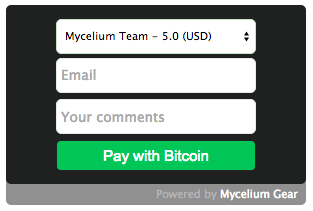
\includegraphics[scale=0.5]{fig/Mycelium_gear.png}
  \caption{Mycelium Gear Widget}
\label{fig:mycelium-widget}
\end{figure}


\textbf{Usability}
Mycelium Gear is designed in a way to suit e-commerce business needs. It should be customized to suit a physical business PoS (User friendly: \prt) . There are no fees related to using this service, the only usability issue is that the BIP32 path\footnote{see ~\ref{BIP32}} that is generated by the PoS widget, sometimes is different with the ones being checked by the mobile wallet client, so there might be some payments missing from the available credits in the application that is actually hard to retrieve if the path is unknown. They offer fast verifications on 0-confirmation transactions (Time-efficient: \full) and it's possible to chose from a list of supported exchanges to retrieve the Bitcoin exchange rate from (Fair exchange rate: \prt). A unique URL is needed to access the payment page and the employees should be aware of this link (Availability: \prt).

\textbf{Deployability}
This method would be simple to implement but somehow more complicated to customize as there's not that much access to the code to be able to customize for business needs. Although the cost-to-run depending on the implementation could be almost zero (Low cost to run: \prt). The only deployability downside is that the payee is forced to use Mycelium Mobile wallet to manage his payments, however doing so makes it easy to use the PoS in other branches and dedicate different accounts to each branch (Enables branching: \full).

 \textbf{Privacy}
As Mycelium Gear uses BIP32 to generate a new address for each transaction request the payees privacy is held (Payee's privacy: \full). However, there is no user management for the report page, If the customer closes the successful payment page, the employee would not be able to check if the payment was received or not unless he has the administrator password to check the transaction list (Confidential Payments list: \prt).

 \textbf{Security}
Nothing related to the PoS holds any private information or keys that might be in danger of getting hacked, so there's no trust in any 3rd party in this sense. Although all the private keys would be in the Mycelium mobile wallet that is not prone to mobile malwares or hardware failure (No 3rd-party trust: \prt ,Data Encryption: \prt) . Also this would be the weak point that if the hacker steals the phone, he has full access to all the available funds and also the future payments if stay unnoticed. The only software dependency is that the user is forced to use Mycelium mobile wallet (No software dependency: \prt)

\subsection{Aunja PoS}
Depending on the requirements, it's possible to use integration of some open source software to build a fully custom self-managed Bitcoin PoS. The details of this custom PoS will be discussed in Section~\ref{Design and Implementation} and the scoring is discussed in Section~\ref{Implementation measurements}.

 \textbf{Usability:}
As this is a fully customized PoS we could use the scenario based requirement engineering method to implement a system that meets the business needs.

 \textbf{Deployability:}
cost-to-run this system depends on the requirements and how it is implemented. There might be some time needed to implement the prototype and change the bugs on the next round of requirement engineering when we get the feedback of the business owner and employees.

 \textbf{Privacy:}
We could implement the system with all the privacy measurements that need to be satisfy for the business owner. New address generation for each transaction would be basic need to have a good private PoS.

 \textbf{Security:}
Same as Privacy, it is possible to keep in mind all the security features when implementing this system. One of the basic needs is that the private keys should not be easily accessible, either kept offline or encrypted if they are stored on the online server and also there should not be any trust in any 3rd party as it is not needed on such a system. Although it should be mentioned that anytime that a third party code is being executed, we are basically trusting the developer for that software. However, in this case all the code used is open source and reviewed.

\subsection{Desicion result}
As you can see in table \ref{tab:method-comp} there is no perfect solution out of the box for a small business to start accepting Bitcoin. After discussing the advantages and disadvantages of each method with the business owner, we decided to implement our own custom PoS using available open source software. This way it would be easy to incrementally change the PoS system with the customer and employees feedback to meet the needs of the business.


\begin{sidewaystable*}

\renewcommand{\arraystretch}{1.3}

\centering

\begin{tabular*}{0.9\textwidth}{@{\extracolsep{\fill}} llccccccccccccc}

\textit{Category} &
\headrow{User Friendly} & 
\headrow{Time-Efficient} &  
\headrow{Fair Exchange Rate} &
\headrow{Availability} &
\headrow{Low Cost to Run} &
\headrow{Enables Branching} & 
\headrow{Maintains Payee's Privacy} &
\headrow{Maintains Payer's Privacy} &
\headrow{Confidential Payments list} &
\headrow{No 3rd-Party Trust} & 
\headrow{Data Ecnryption} & 
\headrow{No Software Dependency} & 
\headrow{ } & % Something about format decay
\headrow{ } \\ \hline 

QRCode 	 				&	&	&\prt	&\full	&\full	&\prt	&	&\prt	&	&\full	&	&\full&&\\
Hardware Terminal 			&\prt	&\full	&\prt	&\full	&	&	&\full	&\prt	&\full	&	&\full	&	&&\\
Online Merchant Services	&\full	&\full&\prt	&\prt	&\prt	&\full	&\full	&\prt	&\prt	&	&\prt	&\full	&&\\ 
Mycelium Gear				&\prt	&\full	&\prt	&\prt	&\prt	&\full	&\full	&\prt	&\prt	&\prt	&\prt&\prt	&&\\ 
Aunja PoS				&\full	&\full	&\full	&\full	&\prt	&\prt	&\full	&\prt	&\full	&\full	&\full	&\prt	&&\\  \hline 


\\
																					
\end{tabular*}

\caption{A comparison of Point of Sale gateways. \full~ indicates the category of client is awarded the benefit in the corresponding column. \prt~partially awards the benefit. Details provided inline.}
\label{tab:method-comp}


\end{sidewaystable*}
  


%==================== Implementation ======================
\section{Design and Implementation}
\label{Design and Implementation}

There are multiple approaches for implementing Aunja PoS. We first have to see what programming language we want to use and under which environment. One of the lower cost methods would be to use a computer on the cafe's network as the web server but the maintenance and support would be really hard as the network might go down, or overwhelmed by the high number of connected devices and would not function properly. Uptime is one of the most important aspects for a payment system. The next low cost solution is to use shared hosting to host the wallet server and design a web based payment interface for the employees and also a reporting page for the business owner to track the Bitcoin payments. This made our decision easier to chose a programming language, the most common programming language supported by most shared hostings is PHP\footnote{PHP originally stood for Personal Home Page, it now stands for PHP: Hypertext Preprocessor\url{https://secure.php.net/manual/en/history.php.php}}. 
\\ \textbf{PHP} is a server-side scripting language designed for web development and can be mixed with HTML to have more tools for interface design. It can be used with MySQL\footnote{Structured Query Language} as the database backend.

\subsection{Implementation measurements}
\label{Implementation measurements}
After multiple rounds of surveying employees and customers to understand their needs and also researching the subject, here is the break down of the results.
\subsubsection{Usability} 
\begin{itemize}

\item \textbf{User Friendly (\full): } The interface should be minimal and simple, with the ability to show the exchange price of Bitcoin to fiat currency, input box for the price in dollars, estimation of Bitcoin amount equivalent to the price and a note section to jot down the details of the transaction.
As for the user facing interface, it should be simple, showing all the required information such as Bitcoin amount, the exchange rate and the QRCode for the deposit Bitcoin address. Both interfaces should indicate when the transaction is complete.

\item \textbf{Time-Efficient (\full): } It should not take more than normal payment system to initiate the payment. A web based interface would have the advantage that it can be loaded from any device with good speed, depending on the Internet speed. Also to verify the payment it should not take a long time. It also need to use fast verification methods to indicate that the payment is propagated (broadcasted to the Bitcoin network). Knowing that a propagated transaction is not same as confirmed transaction but is an accepted risk for low volume transactions.

\item \textbf{Fair Exchange Rate (\full): } After doing our research on this we found the website called Bitcoinaverage\footnote{"BitcoinAverage.com is the first aggregated bitcon price index that was initially launched in August 2013 with a goal to aggregate rates from all available Bitcoin exchanges around the world and provide a weighted average Bitcoin price." \url{https://Bitcoinaverage.com}} that offers a good combination of all the exchange prices to come up with an average daily price to be used as the fair exchange rate. 

\item \textbf{Availability (\full): } The payment interface should be open to public in the sense that it could be loaded on any device.

\end{itemize}
%-------------------------- Deployability --------------------------
\subsubsection{Deployability}
\begin{itemize}

\item \textbf{Low Cost to Run (\prt): } The only costs associated with this implementation would be the annual cost of the shared hosting that nowadays is less than 100 dollars for an unlimited web host. For the sake of this research, there would be no other implementation and development costs.

\item \textbf{Enables Branching (\prt): } For now there's no plan to have more branches for this business, but depending on the implementation, to have another branch it would be as easy as running another instance of the application on the server.

\end{itemize}
 
%-------------------------- Privacy --------------------------
\subsubsection{Privacy} 
\begin{itemize}

\item \textbf{No Information leakage: } The payment interface does not reveal any information about the backend nor the business' internal detail.

\item \textbf{Maintains Payee's Privacy (\full): } There should be a new address generated for each transaction request so no one can see how much the business have received in Bitcoin prior or after each transaction.

\item \textbf{Maintains Payer's Privacy (\prt) : } This would be the payers Bitcoin wallet client responsibility and it would be out of the scope of this PoS system.

\item \textbf{Confidential Payments list (\full): } There should be a reporting and administration interface designed, only accessible to the business owner or designated personals.

\end{itemize}
%-------------------------- Security --------------------------
\subsubsection{Security} 
\begin{itemize}

\item \textbf{No 3rd-Party Trust (\full): } There should not be any sensitive usage of 3rd parties in the system, it should work as a stand alone system.

\item \textbf{Data Encryption (\full): } All the private keys should be encrypted and then stored on the server. 

\item \textbf{No Software dependency (\prt): } There should not be any software dependency on the payment page for the business. The software dependencies on the server side should all be included in the package as open source software. The only piece of software required to use a PoS on a mobile device should be a web browser and we don't consider this as a software dependency.

\end{itemize}


%---------------------------------------------------- Opensource libraries and softwares ----------------------------------------------------

\subsection{Open source libraries and software applications}
There are multiple approaches to implementing the PoS. After the requirement engineering phase, we chose PHP as our main programming language to code this project. This narrows down the options to a few open source projects.
As we examined different PHP Bitcoin projects, we chose the following as the base of our PoS software:

\subsubsection{Bitcoin libraries}
\begin{itemize}

\item \textbf{Bitcoin SCI: }Bitcoin Shopping Card Interface
\item \textbf{PHP Elliptic Curve library\footnote{\url{http://matejdanter.com}}: } Used as a dependency to Bitcoin SCI to generate Bitcoin addresses.
\item \textbf{Bitcoin-prices\footnote{\url{https://github.com/miohtama/Bitcoin-prices}}: } Display Bitcoin prices in human-friendly manner in fiat currency using Bitcoinaverage.com market data

\end{itemize}

After searching the Internet, we decided to use ''Bitcoin SCI: process Bitcoin transactions with PHP'' as the software to use as our Bitcoin core. It is originally designed to be integrated in e-commerce websites but it could be easily modified to meet our needs. 


\textbf{Bitcoin SCI } (Bitcoin Shopping Cart Interface \footnote{\url{http://bitfreak.info/?page=tools&t=bitsci}}): is a set of libraries and tools that enables the user to process Bitcoin transactions with only PHP. 

\begin{figure}[htb!p]
\centering
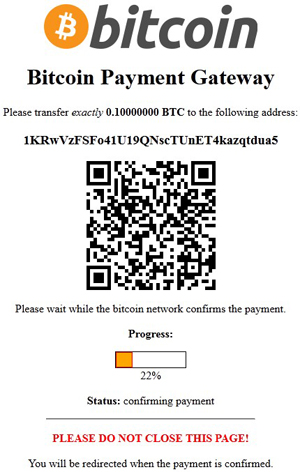
\includegraphics[scale=0.5]{fig/bitsci_screen.jpg}
  \caption{Bitcoin SCI (Bitcoin Shopping Cart Interface)}
\label{fig:Bitcoin-sci}
\end{figure}


This is not a complete project to process payments. The first decision was to use this package for building the prototype and then if we failed to modify the package to meet out needs, use another approach, however we could make it suit the needs and Bitcoin SCI was used in the end product. 

A break down of the tools Bitcoin SCI gives us are as follow:
\begin{itemize}
\item \textbf{Bitcoin Address generation: } Bitcoin SCI uses PHP Elliptic Curve library to generate new secure Bitcoin addresses (set of public and private keys)
\item \textbf{Private key encryption: } using phpseclib library, all the private information (Bitcoin private keys, transaction details) are stored encrypted
\item \textbf{Payment Confirmation: } It uses APIs from a blockchain explorer site \footnote{blockexplorer.com} to confirm receiving payments.
\item \textbf{Input Interface: } even though this package was meant to be used as an e-commerce payment system, it has the basic tools and methods to build the price input page
\end{itemize}

However it lacks some other features that should be added:
\begin{itemize}

\item \textbf{Database: } In order to have management and report page, saving the transaction details into a database is a must.
\item \textbf{Fair Bitcoin Exchange rate: } It uses a predefined source to obtain the exchange rate of Bitcoin and it's not possible to set different currencies as the input
\item \textbf{User-Friendly interface: } All the interfaces are poorly designed and need to be modified to suit the PoS system.
\item \textbf {Report Page: } We need a report page with authentication in place.
\item \textbf {Input Validation: } Other than security perspective of input validation, this is needed because of the way we want the PoS to work. It should alert the employee if she has done something wrong before going to the next page and adding a failed transaction to the database.
\item \textbf {Cash out option: } As all the private keys are stored encrypted in the server, we need a way to cash out the available Bitcoins and send them to another Bitcoin address. It's possible to retrieve the private keys of each Bitcoin address separately from the tool, but it's not scalable to multiple weekly transactions.
\end{itemize}

\textbf{Bitcoin-prices} This library allows us to use Bitcoinaverage.com prices as our main source of price conversion, and it gives nice tools for interface design, such as the ability to switch between different currencies by just clicking on the price. This allows us to reach a fair exchange rate that is also shown in different currencies in case it was needed.

\subsubsection{Encryption libraries}
\begin{itemize}
\item \textbf{phpseclib\footnote{\url{http://phpseclib.sourceforge.net}}: } used for private key encryptions.
\end{itemize}

We used this library mainly because it was already included in the Bitcoin SCI package as a dependency, but later on when we added the database functionality, we needed a library for encryption purposes that they were all included in phpseclib.

\subsubsection{Interface libraries}
\begin{itemize}
\item \textbf{Sweet Alert \footnote{\url{http://t4t5.github.io/sweetalert}}: }  A Beautiful replacement for javascript's ''Alert'', 
\end{itemize}

This is a nice Javascript library that we used to make the interface more user-friendly. Also in the case of data validation, we needed a simple and nice way to inform the employee that she made a mistake on the form and the mistake should be fixed. For this case Javascript is the best option in the sense that it could validate the inputs on the browser before sending it to the server.


%-------------------------- Prototyping --------------------------
\subsection{Prototyping}
With the full knowledge of the requirements and a few sketches of the interface, we started developing the PoS. Although the first prototype was ready to launch within a week, we did 3 prototypes in the month after that, each had bugs fixed and features added as we surveyed and obtained feedback from the employees on each round of prototyping.
\\
Here is a short description of the implemented functionalities:

\subsubsection{PoS main functionalities}
The PoS was hosted on a shared hosting service named Host Monster \footnote{\url{http://hostmonster.com}}. They offer low cost annual plans that offer PHP and MySQL which are the requirements that we need.
Then we started working with Bitcoin SCI to add the database functionality and defined tables for transaction requests and payments on MySQL.

I designed three tables (first prototype had two) for the purpose of this PoS. One table is for the Bitcoin key pairs to be stored and will be used to decrypt and export the private keys when required (see Figure ~\ref{fig:wifkeys}). The other table holds the information regarding each transaction (Figure ~\ref{fig:txhistory}), later on to prevent spam requests and test cases from making the table unnecessary big, we designed a temporary transaction table to hold the data of each transaction before the payment is validated. As soon as the payment is flagged as valid, the relevant data would be moved to the main table and will be removed from the temporary table.

\begin{figure}[htb!p]
\centering
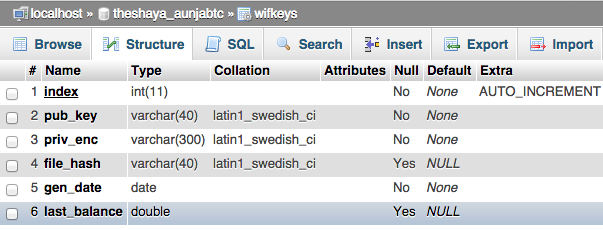
\includegraphics[scale=0.5]{fig/wifkeys_table.png}
  \caption{Structure for wifkeys table that holds the Bitcoin key pairs}
\label{fig:wifkeys}
\end{figure}

\begin{figure}[htb!p]
\centering
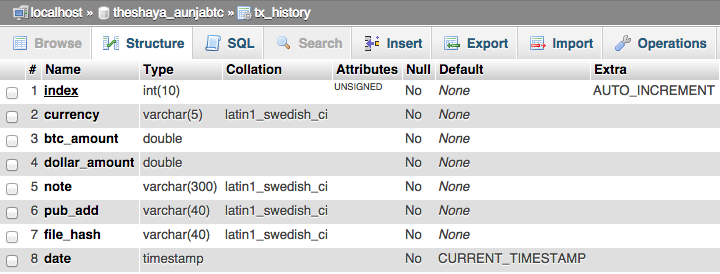
\includegraphics[scale=0.5]{fig/tx_history_table.png}
  \caption{Structure for transaction history table}
\label{fig:txhistory}
\end{figure}

Bitcoin SCI uses a file-based method to store the keys and transaction details, as a backup method, we kept that in place and stored the file\_hash detail of each entity for future references.

Other tasks were involved in integrating the above mentioned open source projects into each other to have a complete solution package.

\begin{figure}[htb!p]
\centering
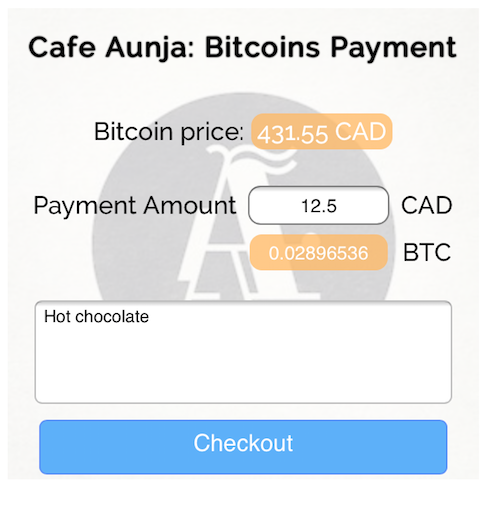
\includegraphics[scale=0.5]{fig/First_View.png}
  \caption{Aunja PoS - First View}
\label{fig:First_View}
\end{figure}

One of the features that were added on the second round of prototyping was the ability to show the Bitcoin price in USD other than the default CAD, this was added with the usage of Bitcoin-prices library. The other was to add the "Notes" field to be able to add invoice ID or the items that the customer bought. It was possible to implement a drop down menu with all the cafe's menu options to be added to the list but as we discussed this solution with the cafe owner, he mentioned that the items in the menu might not stay the same during the year and also there might be price changes, so that approach was not suitable for this business, although it might be a good option for an e-commerce site.

\begin{figure}[htb!p]
\centering
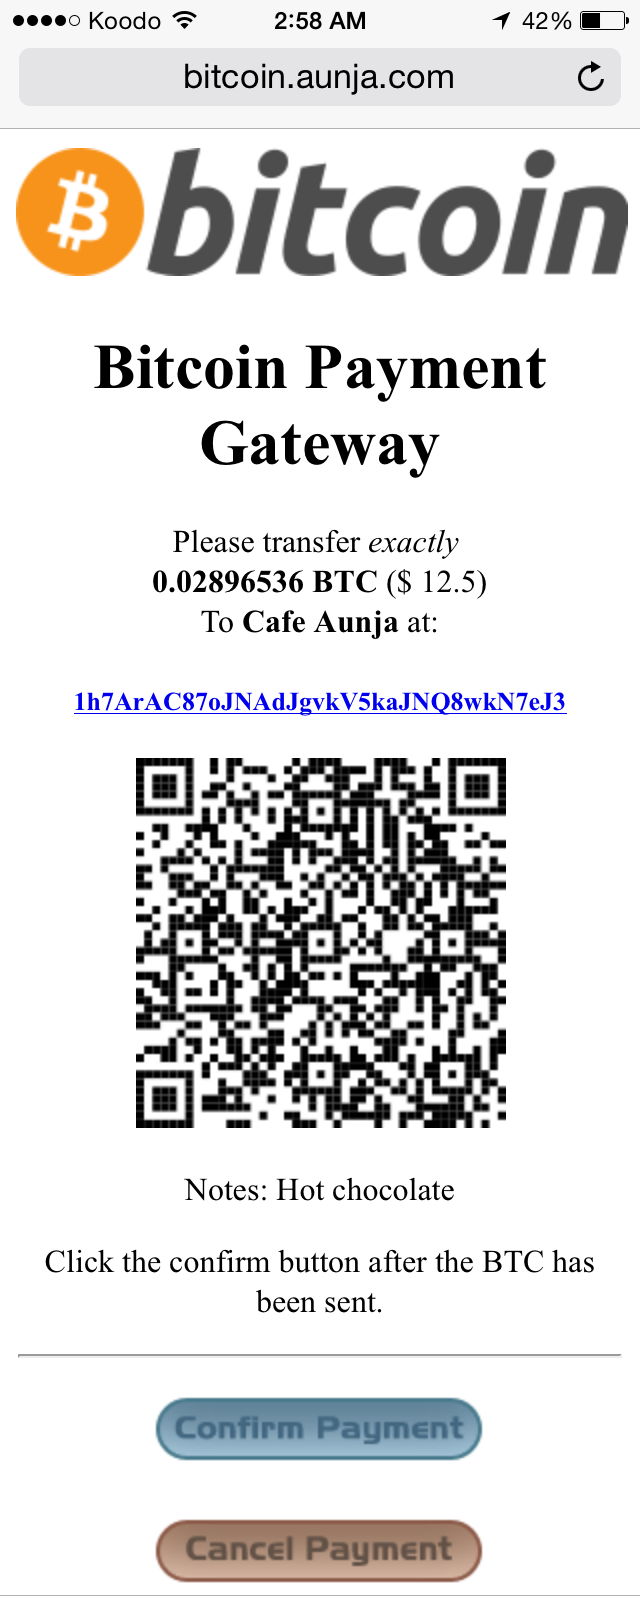
\includegraphics[scale=0.5]{fig/Payment.png}
  \caption{Aunja PoS - Payment}
\label{fig:payment}
\end{figure}

\subsubsection{Private reporting page}
One other aspect of the requirements was a reporting page, this was based on the feedbacks from the cafe's owner and his preferences.

\begin{figure}[htb!p]
\centering
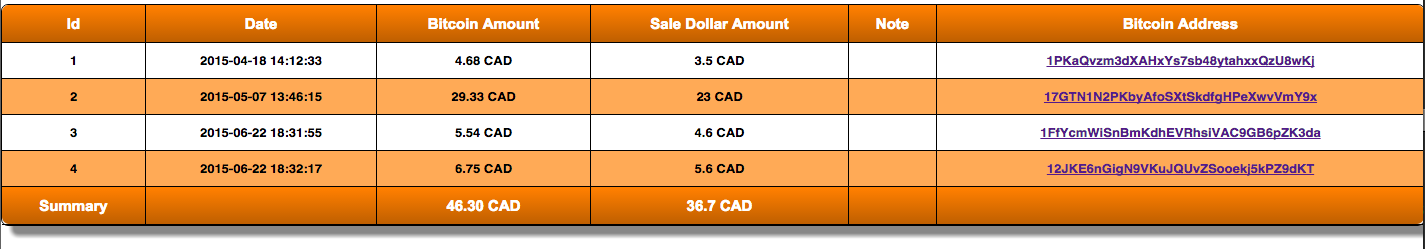
\includegraphics[width=\linewidth]{fig/report_page.png}
  \caption{Report Page}
\label{fig:report_page}
\end{figure}

One of the important fields added later to the report page was the ''Sale Dollar Amount''. The reason was that Bitcoin price is really volatile compared to other currencies and the cafe owner did not want to risk losing money by accepting Bitcoin. As you can see in (Figure~\ref{fig:report_page}), the Sale Dollar amount is less than the Bitcoin amount. In this period of time, the owner could have had more profit on the sales because of the increase in Bitcoin prices, but this would be considered as a risk that he did not want to take. So as an agreement, we decided to lock the price of each sale on the sale time to be paid the same amount as if he was selling his products with cash\footnote{this method is actually one of the common methods recently used by Bitcoin payment processors.}, Thus on the second prototype of the report page, this field was added for accounting purposes. This is real-time exchange, However as an agreement, cashing out the Bitcoins would happen in monthly basis or within a threshold (\eg when reached 100 dollars).

Another added feature was the ability to check each transaction on the blockchain. If the café owner clicks on any of the Bitcoin addresses related to each sale, he would be redirected to a blockchain explorer site and he can see if the transaction went through or not.

\begin{figure}[htb!p]
\centering
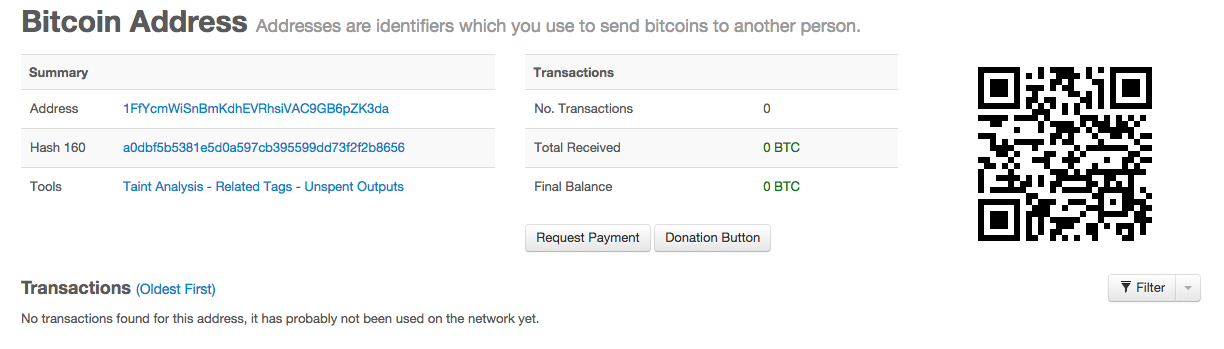
\includegraphics[width=\linewidth]{fig/canceled_sale.png}
  \caption{A canceled sale - this means that the request was made on the Aunja PoS interface to generate an address, but the customer never sent the Bitcoins. Probably a customer changed his mind and paid via another payment method}
\label{fig:canceled_sale}
\end{figure}


\begin{figure}
\centering
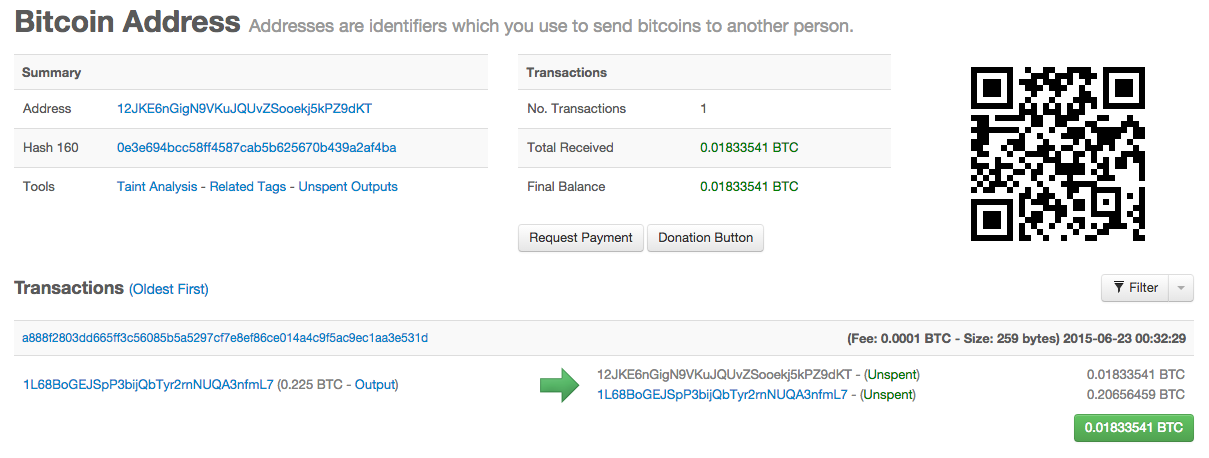
\includegraphics[width=\linewidth]{fig/complete_sale.png}
  \caption{A Complete Sale - This shows that 0.01833541 BTC (approximately 5.5 CAD on the time of sale) was deposited in the address generated by the Aunja PoS} 
\label{fig:report_page}
\end{figure}


Another feature request was the ability to decrypt and export the private keys of those addresses that has some balance. This has been done for the admin page that is out of the scope of this chapter. 

Aunja PoS has been made open source and available to public\footnote{\url{https://github.com/shayanb/Bitcoin-PoS-PHP}} under GNU General Public License v2 and has already been used in other small businesses to accept Bitcoin.

%-------------------------- Training --------------------------
\subsection{Training}

We tried to make the interface as simple as possible for the employees. There is no jargon or technical requirements to use Aunja PoS, but some details specific to Bitcoin transactions have to be taught to the employees to be able to recover from human errors while a transaction is being processed.
Other than in-person training that was done with every employee, a manual was made (Figure~\ref{fig:payment_manual}) and was attached to the cashier's counter for future reference by all café employees.

\begin{figure}[htb!p]
\centering
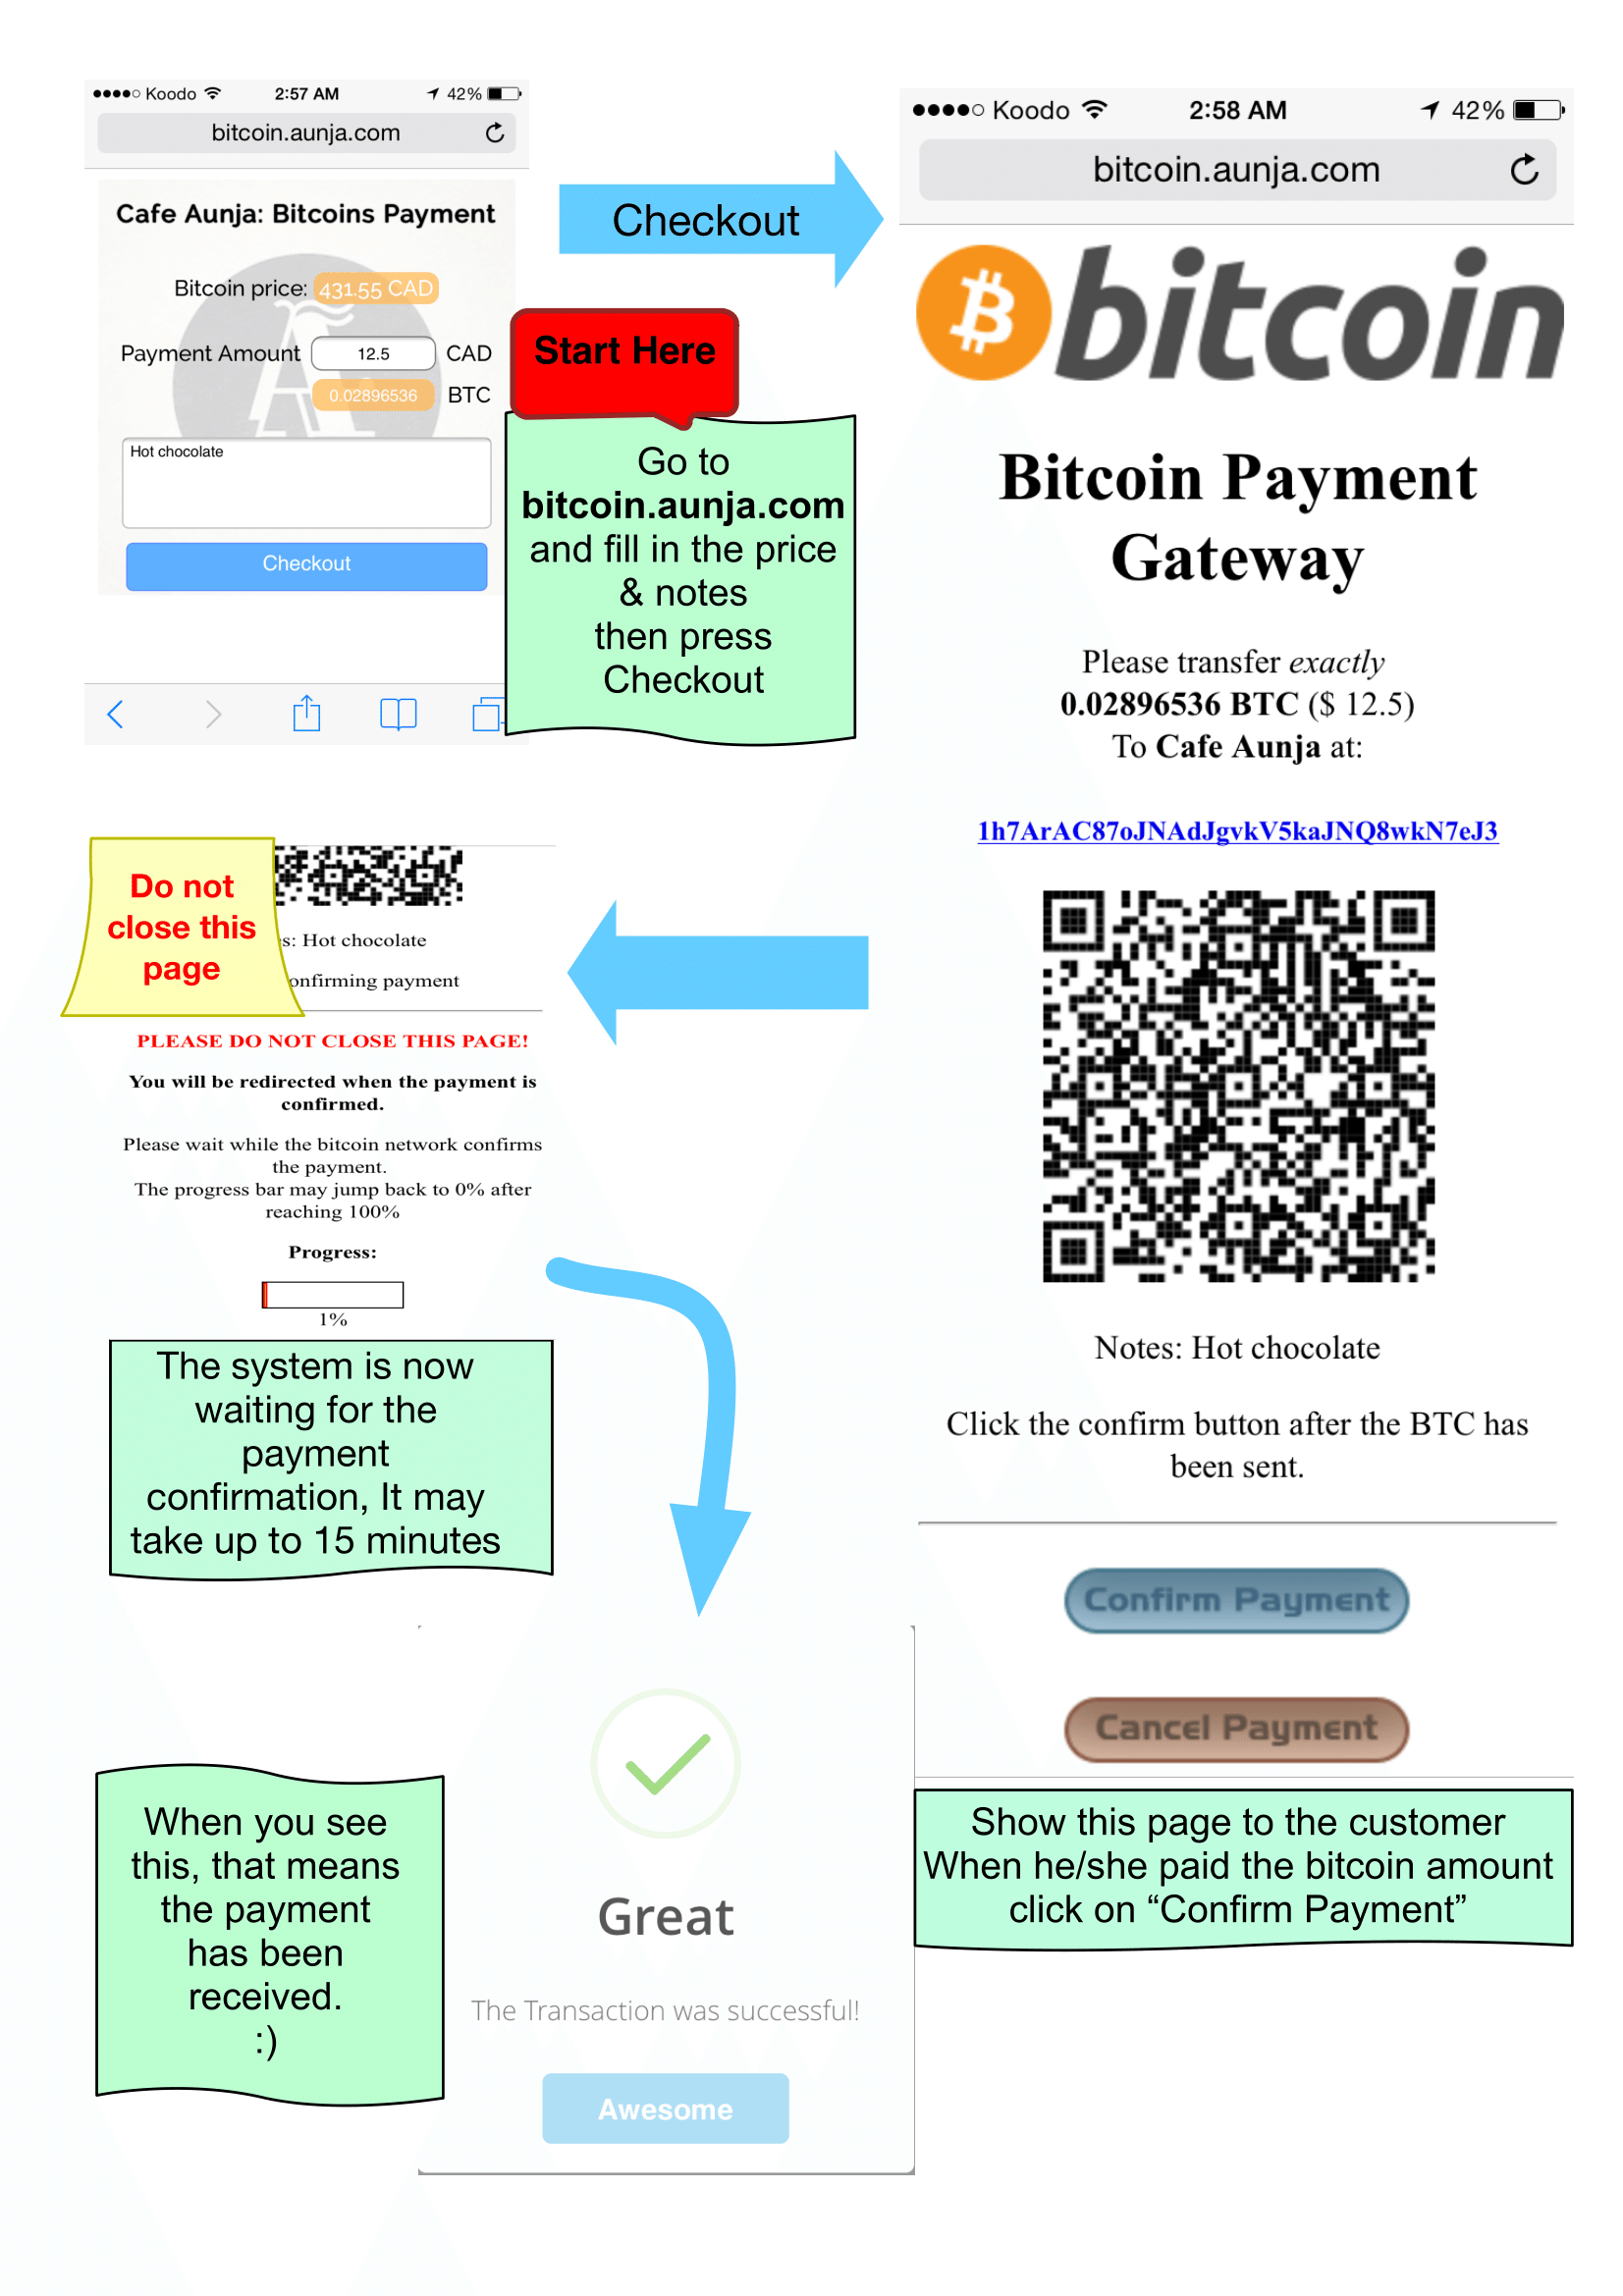
\includegraphics[width=\linewidth]{fig/Payment_manual.png}
  \caption{PoS - Step by step manual for Bitcoin payments}
\label{fig:payment_manual}
\end{figure}



\section{Real-world Deployment}
Café Aunja started accepting Bitcoin with Aunja PoS on Oct 23, 2014, and was one of the first cafés in eastern Canada that accepts Bitcoin. During the first month, there was more than 10 Bitcoin payments and it has been working ever since.

\subsection{Lessons learned}
One of the missing features that should be implemented in such a system is a fast verification method. In early Bitcoin PoS, for each payment, the customer needs to wait 10 minutes in average for the transaction to be confirmed and included in the blockchain. To remedy this, we solved this issue by flagging the transactions as successful as soon as the transaction is broadcasted to the Bitcoin network, also known as, 0-confirmation transaction. This could work for a PoS in a cafe as the volume of each transaction is small and it's not risky to take 0-confirmation transactions, Another newly introduced method to overcome the confirmation time is by using the Bitcoin Lightening Network ~\cite{poon2015bitcoin} but the technical details on lightening network goes beyond the scope of this thesis. However this is still an open problem to remedy the risk for higher value transactions and prevent double spend attacks ~\cite{karame2012two} ~\cite{bamert2013have}. 

Bitcoin and Bitcoin transactions are still new concepts for most people. We encountered a countless number of questions from customers to explain what Bitcoin is and how it works and mostly they became more interested to know more about Bitcoin when they observed a payment done with the Bitcoin PoS, mostly because they would not reveal any personal information with each payment.

Another interesting lesson is the concept of locked price that is the price of Bitcoin for each sale is locked to the exact exchange rate at the time of the transaction. This means if the customer paid 0.01 Bitcoin for a coffee that was 3 dollars in the time of the purchase, the business owner will be paid the exact same amount of 3 dollars and it should not differ if the Bitcoin price has been increasing or decreasing from the time of the purchase to the time he chooses to cash out the receiving Bitcoin. This makes the acceptance of Bitcoin payments for the business risk-free.

Now to test the system on production, it was time for the first coffee, to the best of our knowledge, in eastern Canada to be bought with Bitcoin (Figure ~\ref{fig:firsttransaction}).

\begin{figure}[htb!p]
\centering
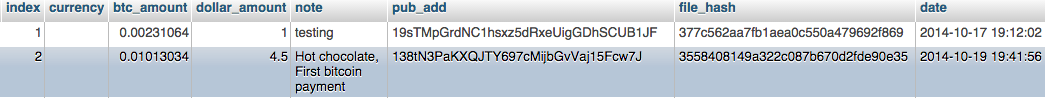
\includegraphics[width=\linewidth]{fig/first_cafe_transaction.png}
  \caption{Database details of the first coffee bought with Bitcoin in the cafe}
\label{fig:firsttransaction}
\end{figure}



\begin{figure}[htb]
\centering
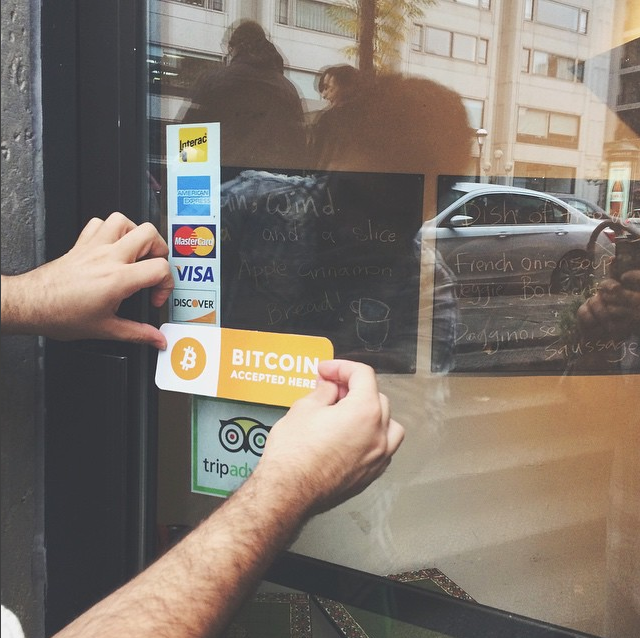
\includegraphics[scale=0.5]{fig/cafeaunja.png}
  \caption{Cafe Aunja Started to accept Bitcoin on Oct 23, 2014 }
\label{fig:cafeaunja}
\end{figure}




